\documentclass[12pt]{beamer}
\usepackage{beamerthemeHannover, graphicx, clrscode, amsmath, amssymb, multicol}
\usepackage{color, verbatim}
\setbeamercolor{sidebar}{use=structure,bg=gray!60!green}
\title{ A Visual Introduction To Parrot Virtual Machine }
\author[@dukeleto]{Jonathan "Duke" Leto \\ Community Manager \\ Parrot Virtual Machine \\ http://parrot.org }
\date{}

\begin{document}

\frame{
    \titlepage
    \begin{center}
%     
\includegraphics[scale=0.5]{parrot_logo}
    \end{center}
}

\frame{
    \frametitle{ What is Parrot, really? }

    Parrot is many things:

    \begin{itemize}
        \item A culture
        \item A collection of languages
        \item A virtual machine to run said languages
        \item A set of tools to write new languages
        \item A playground for research
        \item A second cousin to Perl 6
    \end{itemize}

    Parrot is what you want it to be.
}

\frame{
    \frametitle{ The Parrot Onion }

    ONION diagram
}

\frame{
    \frametitle{ PMC is for Cookie ... }
    PMC = Parrot Magic Cookie a.k.a. Objects \\
    Serious people prefer to call them \\ PolyMorphic Containers

    \begin{center}
     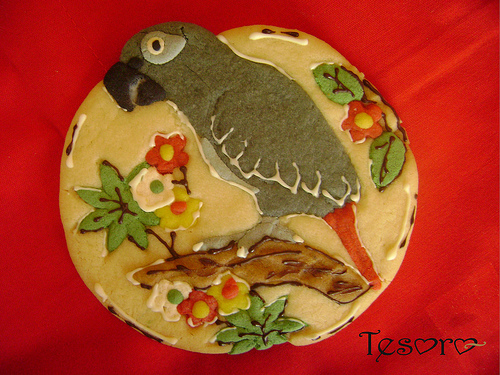
\includegraphics[scale=0.4]{parrot_cookie}
    \end{center}
}

\frame{
    \frametitle{ PMC is for Cookie ... }
    All PMCs follow a "meta-recipe"

    \begin{center}
        \begin{itemize}
            \item \_ cups of \_ flour
            \item \_ \_ eggs
            \item \_ cups of \_ chocolate chips
            \item \_ cups of \_ sugar
            \item \_ sticks of \_ butter
            \item \_ spoons of \_ butter
        \end{itemize}
    \end{center}

    PICTURE OF DELICIOUS COOKIE
}

\frame{
    \frametitle{ PMC is for Cookie ... }

    Some people like really sweet dark chocolate chip peanut butter cookies.

    \begin{center}
        \begin{itemize}
            \item \underline{2} cups of \underline{white} flour
            \item \underline{2 organic} eggs
            \item \underline{1} cup of \underline{dark} chocolate chips
            \item \underline{3} cups of \underline{cane} sugar
            \item \underline{2} sticks of \underline{unsalted} butter
            \item \underline{3} spoons of \underline{peanut} butter
        \end{itemize}
    \end{center}

}

\frame{
    \frametitle{ PMC is for Cookie ... }

    OH NOES! Some people are allergic to peanut butter, dislike processed flour
    and prefer milk chocolate!  Almond butter is a delicious replacement for
    peanut butter.

    \begin{center}
        \begin{itemize}
            \item \underline{2} cups of {\color{red} \underline{wheat}} flour
            \item \underline{2 organic} eggs
            \item \underline{1} cup of {\color{red} \underline{milk}} chocolate chips
            \item \underline{3} cups of \underline{cane} sugar
            \item \underline{2} sticks of \underline{unsalted} butter
            \item \underline{3} spoons of {\color{red} \underline{almond}} butter
        \end{itemize}
    \end{center}

}


\frame{
    \frametitle{ Resources }
    \begin{center}
        \begin{itemize}
            \item http://docs.parrot.org
        \end{itemize}
    \end{center}
}

\frame{
    \frametitle{ Thanks! }
    \begin{itemize}
        \item foo
    \end{itemize}

}

\end{document}
